% install texlive-science to enable algorithm package %

\documentclass{article} % Use the report class instead of article
\usepackage{titlesec}
\usepackage{graphicx}
\usepackage{hyperref}
\usepackage{listings}
\usepackage{color}
\usepackage{amsmath} % Add this line to use \text
\usepackage{tabularx}
\usepackage{algorithm}
\usepackage{tcolorbox}
\usepackage[noend]{algpseudocode}

\definecolor{dkgreen}{rgb}{0,0.6,0}
\definecolor{gray}{rgb}{0.5,0.5,0.5}
\definecolor{mauve}{rgb}{0.58,0,0.82}

\lstset{frame=tb,
  language=Java,
  aboveskip=3mm,
  belowskip=3mm,
  showstringspaces=false,
  columns=flexible,
  basicstyle={\small\ttfamily},
  numbers=none,
  numberstyle=\tiny\color{gray},
  keywordstyle=\color{blue},
  commentstyle=\color{dkgreen},
  stringstyle=\color{mauve},
  breaklines=true,
  breakatwhitespace=true,
  tabsize=3
}

\graphicspath{{./assets/images/}}

\title{%
    
\includegraphics[width=0.3\linewidth]{./assets/logo.pdf}\\[20pt]
    \Huge \bfseries Criptografia aplicada \\[10pt]
    \Large DRSA
}
\author{Tiago Silvestre, 103554 \\ Diogo Matos, 102848}
\date{\today}

\begin{document}

\maketitle

\newpage

\tableofcontents

\clearpage

\section{Introduction}
In the context of RSA key pair generation, sometimes it's necessary to recover the key pair given a human readable set of parameters (e.g password). This process must be computationally hard and deterministic.

So, in this project we developed a pseudo-random byte generator and explored its usage for deterministic RSA key pair generation. 
The generator has a complex and slow setup process to make brute force attacks against it unfeasible. As input the generator receives a password, an iteration count and a confusion string.

The pseudo-random byte generator and rsa key-pair generator were implemented in C++ and in Go. Also, a program was developed in Python to benchmark the setup process of the pseudo random generator.

\section{Implementation}
\subsection{Random byte generator}
The generator state should be computationally hard to achieve and resistant to parallelization. To achieve this, the following steps are taken:

\begin{enumerate}
    \item Compute both the bootstrap seed and pattern.
    \item Iterate over the generator until a pattern is discovered and repeat this process for the specified number of iterations.
\end{enumerate}

The first step involves a memory and CPU-intensive process, while the second step is CPU-intensive. Both of these characteristics make parallelization challenging to achieve.
\subsubsection{Compute bootsrap seed}

To compute the bootstrap seed, the Argon2 algorithm was employed, known for its memory-hard characteristics. Specifically, it utilizes 1GB of memory and uses 3 iterations. This amount of memory was chosen to avoid fast bootstrap seed calculations. Even if the number of iterations is set to a low value, there exists a reasonable lower bound on processing time necessary to determine the final state of the generator.

The pattern is derived from the first bytes of the SHA256 hash of confusion string, dependent on the number of user-requested pattern bytes.

\subsubsection{Find Final Generator State}

Our generator employs the Chacha20 algorithm, known for its ability to generate extensive streams of data based on a predefined state. The algorithm chosen to compute the final seed follows these steps:

\begin{enumerate}
    \item Initialize the generator with the bootstrap seed.
    \item For each iteration, find the first occurrency of the pattern and compute the SHA256 hash of all input until the pattern, including 32 bytes after the pattern.
    \item Initialize the generator with the calculated digest.
    \item Repeat step 2 for the number of iterations specified by the user.
\end{enumerate}

In step 2, it is crucial to ensure that the algorithm has found the seed. Therefore, we request 32 bytes after the seed. Additionally, we ask for the digest of previous bytes until the pattern is discovered. This calculation is necessary because Chacha20 allows random access to stream bytes. By requesting the digest of previous bytes, we ensure that the algorithm has covered the entire stream up to the point where the pattern was discovered.
\subsection{RSA key-pair generator}

This process is followed in order to generate a RSA key-pair:
\begin{enumerate}
  \item Inputs: exponent, $e$, and the key size.
  \item Generate two random prime numbers, $p$ and $q$, with a size equal to half of the key length.
  In order to generete a random prime number, we use our random byte generator to generate
  a value with the needed size, then we perform a primality test, the value 2 is added to the value until it passes primality test;
  OpenSSL's Big Num \textit{BN\_is\_prime\_fasttest\_ex} is used to perform the primality test. It starts by making a trial division by a set of
  small prime numbers and then at least 128 rounds of Miller-Rabin. This is considered a probability
  test that performs multiple checks to see if the number is composite, if all return negative, the number is considered prime. The process of 
  prime generation has a $2^{-256}$ false positive rate.
  \item Compute $n$, $n=p*q$;
  \item Compute Carmichael's totient function, $y(n)$, for that we compute $$y(n)=\frac{(p-1)(q-1)}{\gcd((p-1),(q-1))}$$.
  After the computation, we check the condition $$gcd(e, y(n)) = 1$$, if false we do not proced;
  \item Compute $d$, the modular inverse, $$d=e^{-1} \bmod{y(n)}$$;
  \item $n$, $e$, $d$, $p$ and $q$ are the private key. $n$ and $e$ are the public key.
\end{enumerate}

In order to export the PEM formated public/private keys, RSA key object is initialized, in Go using the Crypto library and in C++ using OpenSSL.

For OpenSSL the Chinese remainder theorem related constants, $dmp1$, $dmq1$ and $iqmp$, need to be computed as well:
$$dmp1=d \bmod{(p-1)}$$, $$dmq1=d \bmod{(q-1)}$$, $$iqmp1=q \bmod{p}$$

With that, $n$, $e$, $d$, $p$, $q$, $dmp1$, $dmq1$ and $iqmp1$ are the private key. $n$ and $e$ are the public key.

\section{Discussion}
\subsection{Generator security}

Given that the generator is based on ChaCha20, its security (after the setup is done) is the same as ChaCha20 (known to be safe). Besides that, some tests were made to ensure that small variations in input arguments produced distinct outputs \texttt{cpp/test\_RBG.cpp}.

To support the safety of the setup process, the usage of Argon2 allows us to conclude that finding the bootstrap seed is both memory and computationally a hard process. Also, the calculation of SHA256 with the bytes until the pattern is found guarantees that this process cannot be fully paralelized (only finding the pattern is) but computing the hash it's harder and it's done in a single thread.

Also, for low iterations we wanted to keep the process hard, so we decided to use Argon2.
\subsection{Generator setup time}
In order to make brute force attacks unfeasible, the bootstrap process shall be very dependent on the input parameters and have slow setup process.

\begin{figure}[!ht]
  \label{figure:apache_headers}
  \centering
  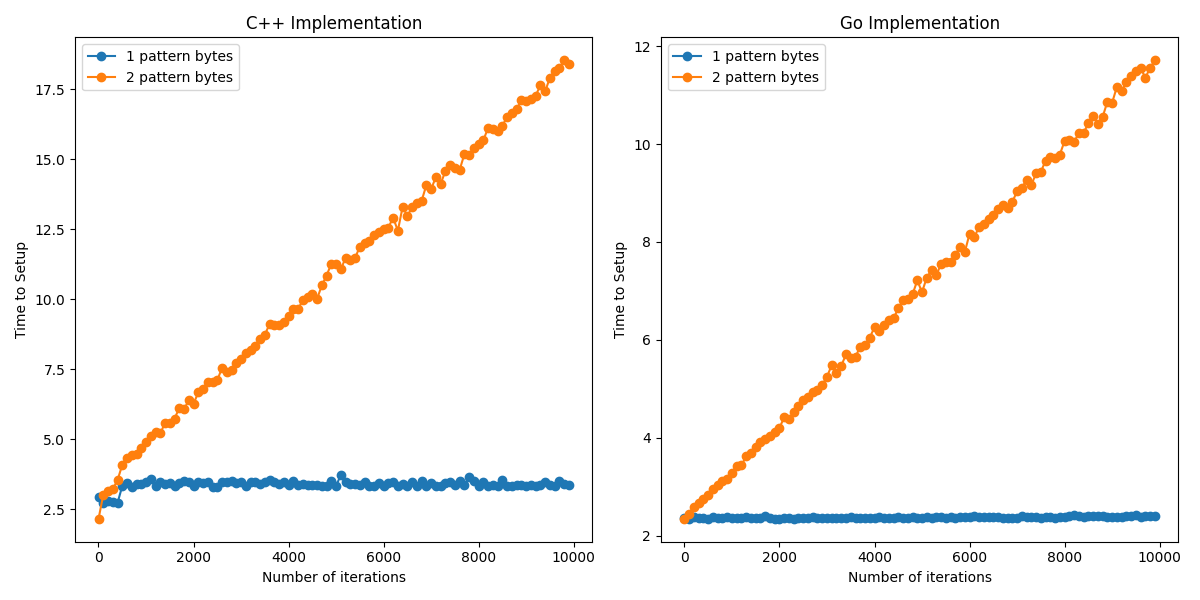
\includegraphics[width=0.7\textwidth]{assets/randgen_plot1.png}
  \caption{Setup time for a number of pattern bytes between 1 and 2, and number of iteration between 1 and 10000.}
\end{figure}

As we can see the time to setup the generator goes up with the number of pattern bytes and number of iterations. Of course, when using 
just one pattern byte, the number of iterations does not make much difference, because its very fast to generate a given byte. The number pattern bytes
should be two or three, more than that the setup takes an unusable (for most use cases) amount of time to setup. Even with three pattern bytes, takes too long
to be includes in the plot above.

For example, to test all possibilities for 4000 iterations and a two pattern bytes using the Go Implementation, it would take $1.9 \times 10^{74}$ minutes. About $8 \times 10^{72} days$.
This value is good enough to the a brute force attack to be unfeasible.


\section{Conclusions}
A pseudo-random random generator was developed with a secure setup process was developed and integrated for RSA key pair generation, succesfully.

\end{document}
